\documentclass[11pt]{article}
\usepackage{amsmath,bm,amsfonts,color,amsthm}
%\usepackage[margin=2.5cm]{geometry}
\usepackage{graphicx}

\usepackage[compress]{natbib}
\usepackage{comment}
\bibpunct{(}{)}{;}{a}{}{,}
\usepackage[colorlinks,citecolor=blue,urlcolor=blue]{hyperref}
\usepackage{lineno}
\linenumbers
\usepackage{booktabs}
\usepackage{setspace}
\usepackage[ruled,lined]{algorithm2e}
\usepackage{float}
%\usepackage[utf]{arabxetex}
\usepackage{mathtools}	

%\newfontfamily\arabicfont[Script=Arabic]{Amiri}


%\floatstyle{boxed}
\restylefloat{figure}
\SetKw{KwSet}{Set}
%\doublespacing
	
%\setlength{\parskip}{10pt plus 1pt minus 1pt}

% \usepackage{tikz}
% \usetikzlibrary{decorations.pathmorphing} % noisy shapes
% \usetikzlibrary{fit}         % fitting shapes to coordinates
% \usetikzlibrary{backgrounds} % drawing the background after the
%                              % foreground
% \usetikzlibrary{positioning}
% \usetikzlibrary{shadows}
% \usepgflibrary{shapes}
% \tikzstyle{observed}=[circle, thick, minimum size=0.7cm, draw=black!100, fill=black!20]
% \tikzstyle{latent}=[circle, thick, minimum size=0.7cm, draw=black!100]
% \tikzstyle{plate}=[rectangle, thick, inner sep=0.3cm, draw=black!100]
% \tikzstyle{shadeplate}=[rectangle, thick, inner sep=0.3cm, draw=black!100, fill=black!10]

\DeclareMathOperator*{\argmin}{argmin}



\title{Locality Sensitive Hashing}
\author{Rebecca C. Steorts}
\date{\today  }
\begin{document}
\newcounter{itemnum}
\newtheorem{lemma}{Lemma}
\newtheorem{theorem}{Theorem}
\newtheorem{corollary}{Corollary}

\theoremstyle{definition}
\newtheorem{definition}{Definition}
\newtheorem*{remark}{Remark}

\newtheoremstyle{lemma}
{\topsep} % space above
{\topsep} % space below
{\it} % body fontt
{} % indent
{\bf} % head font in lower caps bolded
%{\sc} % head font in all caps not bolded
{:} % punctuation between head and body
{0.5em} % space after head
{} % manually specify head
%{\thmname{#1}\thmnumber{ #2}\thmnote{:#3}} % manually specify head
%\newtheorem{theorem}{Theorem}
\theoremstyle{lemma}
\newtheorem{lem}{Lemma}

%\input{symbols}

\maketitle




\section{Locality Sensitive Hashing (LSH)}

A {\em hash function} maps objects to integers such that
dissimilar objects are mapped far apart.  LSH uses special hash functions to
ensure that similar objects are put close to each other (with high
probability).  By applying several locality-sensitive hashes to a record, one
goes from a high-dimensional object to a low-dimensional signature, with a
guarantee that similar records have nearby signatures.  The low-dimensional
signature vectors can then be divided into bins or blocks, with a high
probability that all records mapped to the same bin are similar, and a hope
that not too many similar records fall into different bins.  If the number of
records per bin is small, we can treat the bins as blocks for purposes of
record linkage.  The number of records per bin depends on the exact binning
procedure and its tuning parameters \citep{kim_2010, rajaraman_2012,
  christen_2011}.  Unlike conventional blocking, LSH uses all the fields of a
record and can be adjusted to ensure that blocks are manageably
small.\footnote{The last point needs some care, since simulation studies show
  that \emph{sometimes} bins can contain many records, leading to minimal
  computational savings.}  By design, records falling within the same block are
similar to each other, so only linking records within blocks can lead to
dramatic speed-ups while imposing only a small cost in false negative errors.
(One does fewer comparisons, and those comparisons are more likely to lead to
links.)

While these are all desirable features, LSH is in several ways not yet fully
developed as a blocking technique for entity resolution.  One is that
``similarity'' must be made computationally precise, and not every similarity
measure is preserved by a (known) family of hash functions.  Moreover,
different similarity measures may be appropriate for different kinds of data
in different applications.  Second, entity resolution should come not from
ranking similarity scores \citep[as in][]{christen_2014}, but from a
statistical model. We develop a variety of LSH blocking algorithms which are
designed to work well with real-world examples of entity resolution and to
meet the needs of my statistical models.

%\subsection{K-means LSH}
%
%We review the approach of KLSH proposed by \cite{steorts_2014_hash}. LSH-based blocking schemes ``shingle''
%\cite{rajaraman_2012} records.  That is, each record is treated as a string and
%is replaced by a ``bag'' (or ``multi-set'') of length-$k$ contiguous
%sub-strings that it contains. These are known as ``$k$-grams'', ``shingles'',
%or ``tokens''.  The string ``TORONTO'' yields the bag of length-two
%shingles ``TO'', ``OR'', ``RO'', ``ON'', ``NT'', ``TO''.  (N.B., ``TO'' appears
%twice.)
%
%As an alternative to shingling, we might use a bag-of-words representation, or
%even to shingle into consecutive pairs (triples, etc.) of words. 
%In our
%experiments, shingling at the level of letters works better than dividing by
%words.
%
%KLSH starts 
%by shingling the records, treated as strings. KLSH does not ignore the number of times each shingle type appears in a
%record, but rather keep track of these counts, leading to a bag-of-shingles
%representation for records.   Similarity is measured between
%records using the inner product of bag-of-shingles vectors, with
%inverse-document-frequency (IDF) weighting. 
%Dimensionality is reduced of the bag-of-shingles vectors by random projections, followed
%by clustering the low-dimensional projected vectors with the $k$-means
%algorithm. 
%% \textcolor{blue}{Notation clash: $k$ for length of shingle vs.\ $k$
%%  for number of clusters.  Need to fix?}  
%Hence, we can control the mean
%number of records per cluster to be $n/c$, where $c$ is the number of block-clusters.  In practice, there is a fairly small
%dispersion around this mean, leading to blocks that, by construction, have roughly the same distribution for all applications.\footnote{This property is not guaranteed for most LSH methods.}  The KLSH algorithm is given in Appendix \ref{sec:app}.

\subsection{Minwise hashing}

Minwise hashing is a procedure for comparing the similarity of two sets (records in this context can be thought of as sets). For a large dataset like the Syrian one we are considering, minwise hashing is optimal because of its speed in subdividing records into blocks. The implementation of minwise hashing has a number of steps.

\begin{description}
\item[First] \hfill \\
We shingle each record. Shingling is a way of splitting apart a record into smaller subsets, at some specified splitting point. For example, if we have the record [``Peter", ``Pittsburgh"], and we want to use a shingling of size k = 3, we form the shingles [``Pet", ``erP", ``itt", ``sbu", ``rgh"]. To do this, we combine the entire record into a single string, and then subdivide it into parts of three.

Shingling is done to each record in the dataset, which forms a large set of shingles. We also want to keep track of which records are associated with which shingles. So if we have a second record, [``Steve", ``Pittsburgh"], then we know that the shingles ``itt", ``sbu", and ``argh" are in common between the two records.

\item[Second] \hfill \\
We form a characteristic matrix from the shingles. A characteristic matrix is an indicator matrix, where the columns of the matrix correspond to records in the dataset (so there is a column for each record) and the row to the shingles formed from the records (so there is a row for each shingle). The elements of the matrix are a binary (1, 0) decision, where a 1 is present if the record contains the corresponding shingle, and a 0 if not. The characteristic matrix is very sparse (i.e., it contains mainly 0s), as most records do not contain the majority of all possible shingles.

Table 1 is an example of a characteristic matrix, with four records(sets) and five shingles(elements). 

\begin{table}[h]
\begin{center}
\begin{tabular}{@{}lllll@{}}
\toprule
Element 1-5 & $S_{1}$ & $S_{2}$ & $S_{3}$ & $S_{4}$ \\ \midrule
1   & 0       & 0       & 1       & 1       \\
2   & 1       & 0       & 0       & 1       \\
3   & 1       & 1       & 0       & 0       \\
4   & 0       & 0       & 0       & 1       \\
5   & 1       & 0       & 0       & 1       \\ \bottomrule
\end{tabular}
\label{table:samplemat}
\caption{A sample characteristic matrix, with four records in columns and five possible shingles in rows. As the number of shingles grows, the matrix becomes increasingly sparse, as most records do not contain most shingles.}
\end{center}
\end{table}

\item[Third] \hfill \\
We permute the rows of the characteristic matrix to form a permuted matrix. If we have five rows, 1-5, then possible permutations of the rows are 12345, 15234, and 54321 (there are many others). The permuted matrix, then, is simply a reordering of the original characteristic matrix, with the rows swapped in some arrangement. Figure \ref{fig:permuted} shows the characteristic matrix converted to a permuted matrix by a given permutation.

We repeat the permutation step for several iterations to obtain multiple permuted matrices. 

\begin{figure}[!h]
\begin{center}
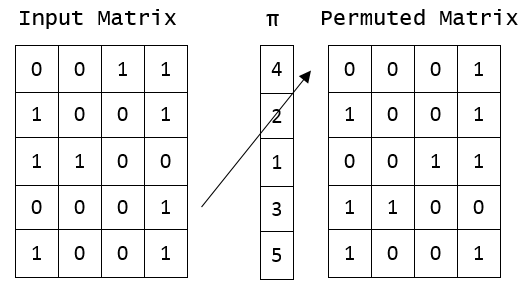
\includegraphics[width=0.8\textwidth]{permuted-matrix.png}
\label{fig:permuted}
\caption{Permuted matrix from the characteristic one. The $\pi$ vector is the specified permutation.}
\end{center}
\end{figure}

In practice, the implementation of minhashing is slightly different from these permutations, as permuting the matrices a large number of times is computationally-prohibitive. To make up for this, a series of hash functions is generated, where the hash function assign values to each row, in exactly the same way as the permutations do. The hash function, $(r + 1) \% 5$, for example, takes in a row index (1-5), and assigns the new indices as the permuted matrix. This results in the same outcomes as the one above. An example of these hash functions with the characteristic matrix is given in table 2.

\begin{table}[h]
\begin{center}
\begin{tabular}{@{}ccccc|cc@{}}
\toprule
Row & $S_{1}$ & $S_{2}$ & $S_{3}$ & $S_{4}$ & (r+1) \% 5 & (3r+2) \% 5 \\ \midrule
0   & 0  & 0  & 1  & 1  & 1          & 2           \\
1   & 1  & 0  & 0  & 1  & 2          & 0           \\
2   & 1  & 1  & 0  & 0  & 3          & 3           \\
3   & 0  & 0  & 0  & 1  & 4          & 1           \\
4   & 1  & 0  & 0  & 1  & 0          & 4           \\ \bottomrule
\end{tabular}
\label{fig:hash-mat}
\caption{Characteristic matrix with four sets, two hash functions, and a generated binary matrix. The hash values are found by inputting the corresponding row index to the hash function.}
\end{center}
\end{table}

\item[Fourth] \hfill \\
We compute the signature matrix. The signature matrix is a hashing of values from the permuted one. The signature has a row for the number of permutations calculated, and a column corresponding with the columns of the permuted matrix. We iterate over each column of the permuted matrix, and populate the signature matrix, row-wise, with the row index from the first 1 value found in the column. The row index inputted to the signature matrix is the new row index the row was associated with, rather than the original index value. The signature matrix for table 1 is in table 3.

\begin{table}[h]
\begin{center}
\begin{tabular}{@{}lllll@{}}
\toprule
        & $S_{1}$ & $S_{2}$ & $S_{3}$ & $S_{4}$ \\ \midrule
$h_{1}$ & 2       & 4       & 3       & 1       \\ \bottomrule
\end{tabular}
\label{fig:signature}
\caption{Signature matrix formed from table 1. The value for each element is the row index in which the first 1 is found in the permuted matrix.}
\end{center}
\end{table}

\item[Fifth] \hfill \\
Based on the results of the signature matrix, we observe the pairwise similarity of two records. For the number of hash functions, there is an interesting relationship that we use between the columns for any given set of the signature matrix and a Jaccard Similarity measure.

The Jaccard Similarity, which is a measure of similarity, is fundamental in this approach. For two sets S and T, the Jaccard Similarity is given by $$\frac{|S \cap T|}{|S \cup T|}$$ which is the intersection of the two sets over their union. It provides a sense of how much two records agree in their fields, over their total number of variables.
   
The relationship between the random permutations of the characteristic matrix and the Jaccard Similarity is:

$$Pr\{min[h(A)] = min[h(B)]\} = \frac{|A \cap B|}{|A \cup B|}$$

The equation means that the probability that the minimum values of the given hash function, in this case $h$, is the same for sets A and B is equivalent to the Jaccard Similarity, especially as the number of record comparisons increases. The output of this formula, in terms of the signature matrix, can be seen in figure \ref{fig:permuted}.

\begin{figure}[htbp]
\begin{center}
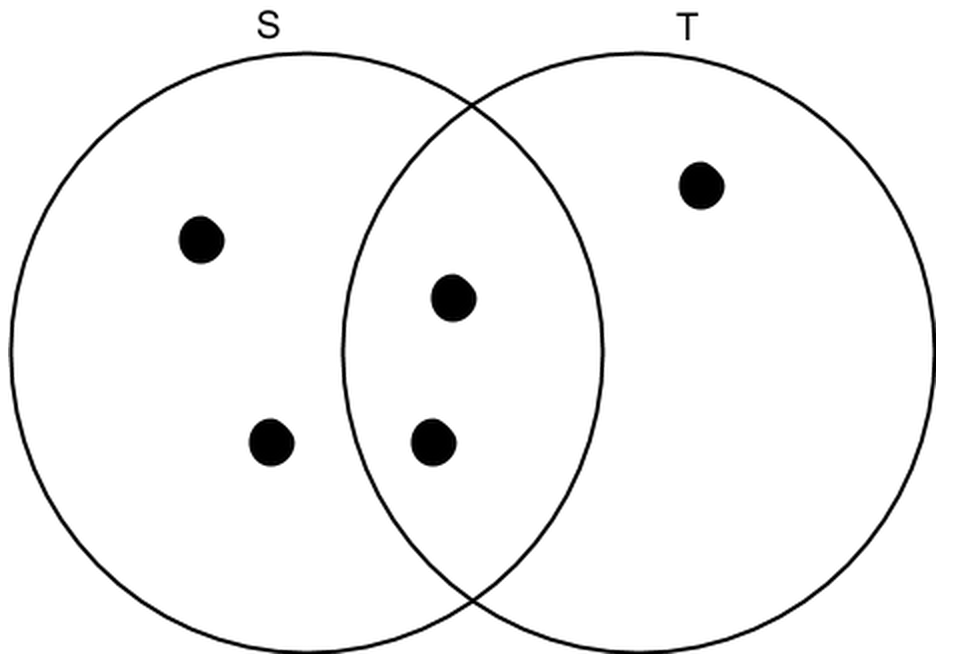
\includegraphics[width=0.5\textwidth]{jaccard.png}
\caption{Two sets S and T with Jaccard similarity 2/5. The two sets share two elements in common, and there are five elements in total. }
\label{fig:jaccard}
\end{center}
\end{figure}

We use this relationship to calculate the similarity between any two records. We look down each column, and compare it to any other column: the number of agreements over the total number of combinations is equal to Jaccard measure.
 	
\end{description}

Of course, in practice, we would need to repeat the above for many permutations $\pi$ such that we avoid collisions, or mapping the different records into the same bin. 

Notice that we have walked through a very elementary view of locality sensitive hashing, and we still have the limitation that we are having to do all-to-all comparisons. How do we avoid this?

\section{LSH for Minhash Signatures} 
See Section 3.4.1 in Mining for Massive Datasets and work through the exercises (some of these we did in class). 
See Example 3.11 and Exercise 3.4.1 and 3.4.2. 

\section{Further reading}
For further reading about hashing and it's use in practice, please refer to \url{https://arxiv.org/abs/1710.02690}. 

\section{Overview of Locality Sensitive Hashing (LSH) Algorithm}
Below we outline the LSH algorithm (for all-to-all comparisons) and also for filtering out documents that are not very similar. 

\begin{enumerate}
\item Construct shingles of all documents in your corpus.
\item Hash all of your shingled documents. 
\item Compute pairwise Jaccard similarity coefficients for all documents.
\begin{enumerate}
\item To do this in a computationally more efficient way, use the characteristic matrix and a random permutation. 
\item Then create the signature matrix by using the minhash. Repeat this process using many random permutations in order to avoid collisions. This will increase the size of your signature matrix. 
\end{enumerate}
\end{enumerate}
To avoid performing all-to-all comparisons as in the above situation, we compute the Jaccard similarity only for candidate pairs using $b$ bands and $r$ rows of the signature matrix, which provide a threshold $t= (1/b)^{1/r}$ using the steps above but now using these extra conditions of filtering out documents that are unlikely to be the same. 





\small{
\bibliography{chomp}
\bibliographystyle{ims.bst}
}





\end{document}